\subsection{Oracle Portal to WCM migration}

This document will go over the basic information needed to become
fluent in using Oracle Web Content Management.  This document is
targetted at any department who needs to move their web site from the
legacy Oracle Portal to the new Oracle UCM infrastructure.

\subsection{Migration Overview}

Your department will have a URL(s) that are designated as your
departments new Web Content Management(WCM) site.  Some of you will
have the responsibility/permission to update your departmental web
site.  How these web pages are updated, and other related WCM concepts
will be conveyed in this document.

\subsection{Website Searching}
 
There are several important web sites that you need to be aware of.

\begin{tabular}{|l l|} 
\hline
Web Site           & Function \\
\hline 
my.oracle.com      & Corporate home page \\ 
content.oracle.com & Corporate Content Management System \\ 
search.oracle.com  & Corporate Search Engine \\
\hline
\end{tabular}


When you update your content on your web site, that content will then
become searchable from the Corporate home page.  If we go to the URL:

\begin{verbatim}
http://my.oracle.com/site/japan/index.htm
\end{verbatim}

We can see the text: ``MyOracle Japan (Employee Portal for Oracle
Japan)'' there.  Next we can navigate to:

\begin{verbatim}
http://my.oracle.com
\end{verbatim}

\begin{figure}[h!]
  \centering
  \fbox{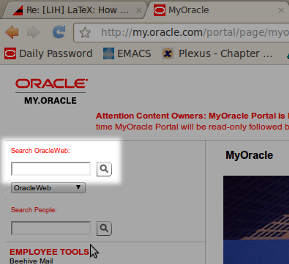
\includegraphics{images/myoracle_search}}
  \caption{my.oracle.com Search box.}
\end{figure}

and in the ``Search OracleWeb'' on the top left we can put the
following in: ``MyOracle Japan Employee Portal for Oracle Japan'', and
press search.  We notice that the top hit is indeed:
``http://my.oracle.com/site/japan/index.htm''.

r\begin{figure}[h!]
  \centering
  \fbox{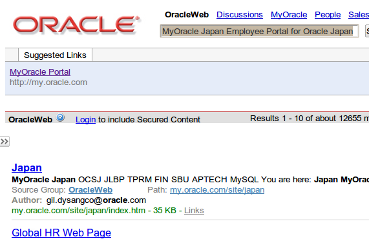
\includegraphics{images/searchResults}}
  \caption{Search results.}
\end{figure}

So that is how content you update directly on your departmental web
site becomes globally accessible.

Now we will take a moment to discuss some general Content Management principles.
\begin{figure}[h!]
  \centering
  \fbox{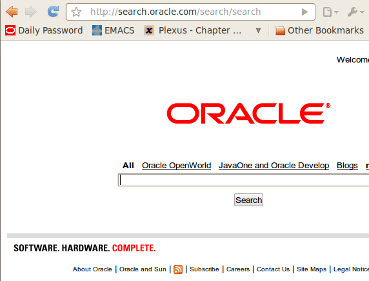
\includegraphics{images/searchOracleCom}}
  \caption{Oracle Search (SES)}
\end{figure}


